\section{Mars Colonization}

\begin{figure}
\centering
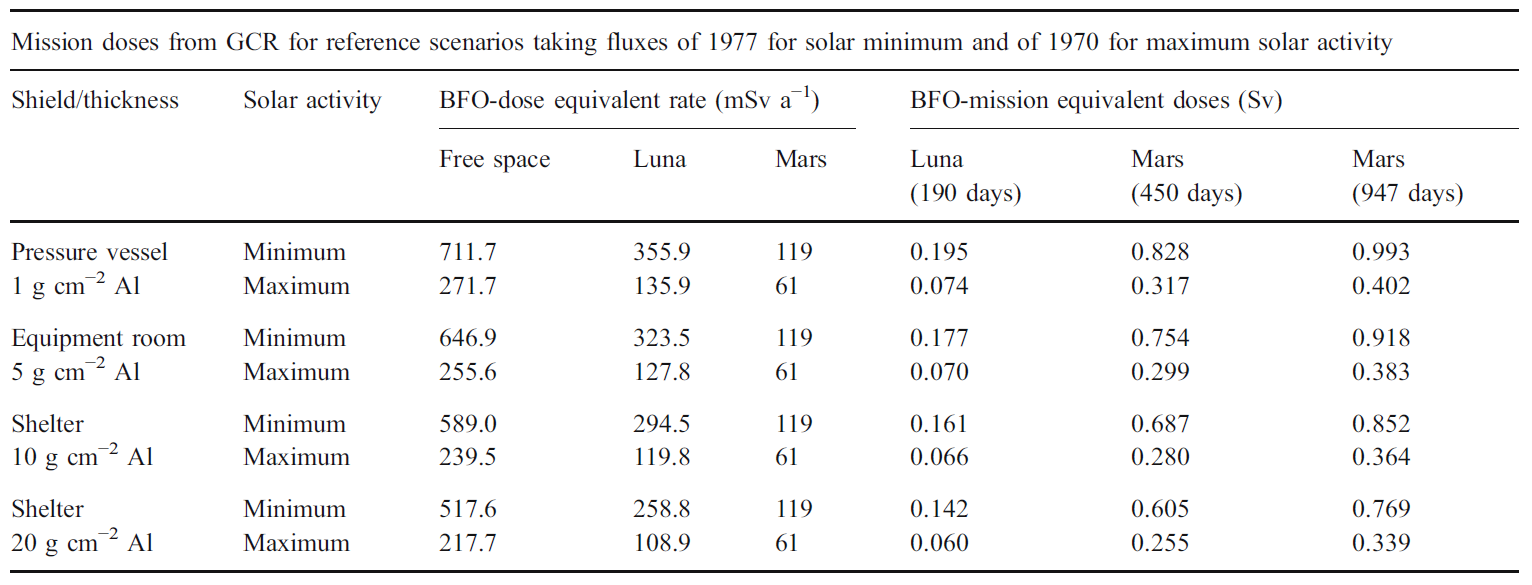
\includegraphics[width=\linewidth]{hellwig-doses.png}
\caption{Radiation doses due to GCRs for several space exploration mission scenarios \cite{hellwig-estimates}. Notice that the vast majority of dose received would be in deep space transit to Mars. While the cumulative doses are very large compared to existing or past LEO or Moon missions, it would be possible to keep radiation exposure below career limits set by NASA and NCRP.}
\label{fig:hellwig}
\end{figure}

\begin{figure}
\centering
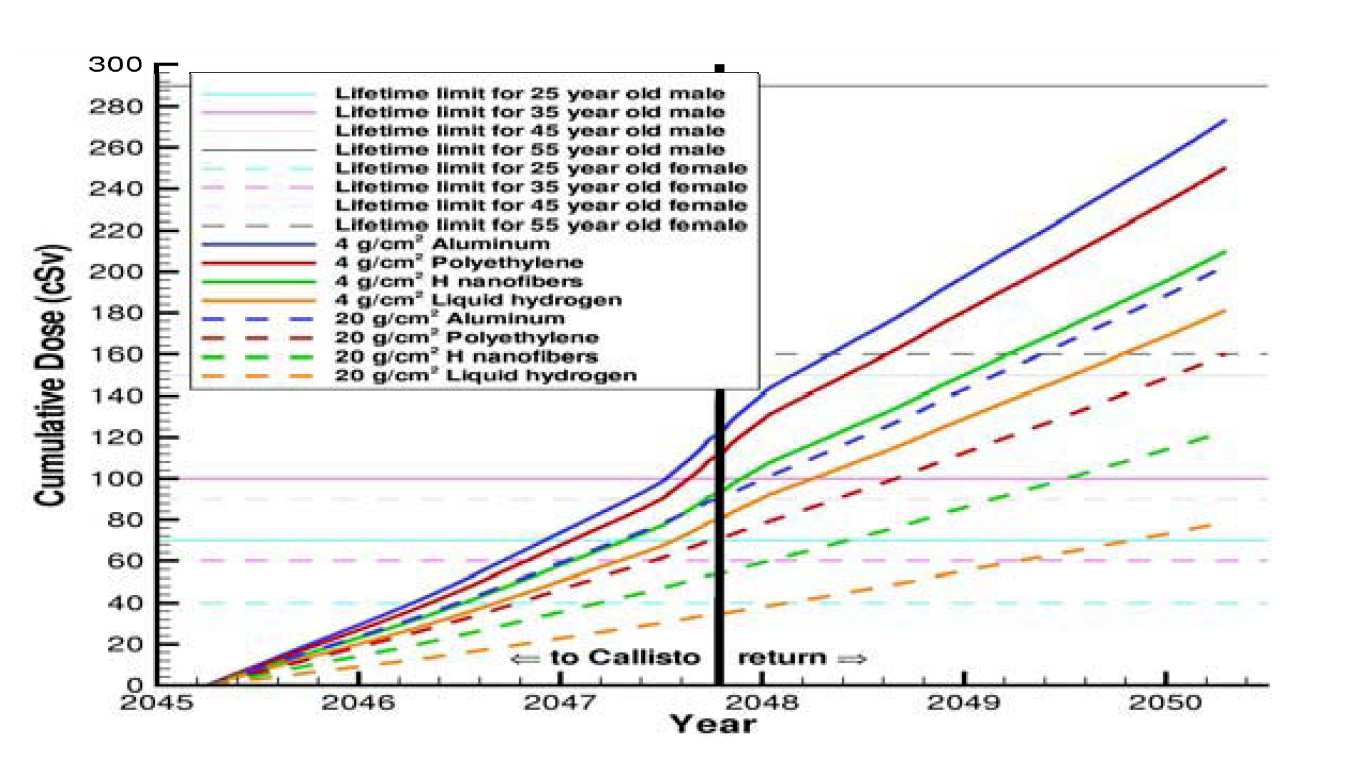
\includegraphics[width=\linewidth]{deangelis-doses.png}
\caption{Predicted cumulative doses over the concievable timeframe of a deep space exploration mission to Jupiter/Callisto \cite{deangelis-scenarios}. Doses are subdivided by sex, age, and different shielding material strategies. Notably while the total doses are high, they are still manageably within career limits.}
\label{fig:deangelis}
\end{figure}

The estimated radiation dose received during a half-year visit to the ISS is 0.075 Sv. To highlight the challenge scientists face with landing humans on Mars, the estimated dosage in-transit to Mars could be over six times as much \cite{kerr-mars}.This problem is further complicated by the variability in a Mars mission (i.e. planetary touchdown versus fly-by missions). Transit to the red planet will be longer and more exposed than travelling to the Moon or LEO. In addition, just as Earth traps particle radiation in its magnetic field, so too does Mars. Moreover, the intention of sending humans to Mars is to ultimately establish a permanent planetary base. Permanent human colonization of Mars increases the value in long transit times and provides scientific and economic advantages to the mission. However, this also increases the complexities of designing equipment since shielded planetary structures need to be developed as well as spacecraft. While Mars possesses an atmosphere that can shield against GCRs, this atmosphere is far weaker and its environment is vastly different than Earth’s and must be considered independently.

The first step in developing a Martian shielding strategy is to quantify the entire mission dosage. This has historical been difficult since technology did not allow direct measurement of radiation levels. Traditionally, radiation transport codes have been used to simulate the expected radiation levels in deep space and on Mars \cite{simonsen-transport}. Taking these simulated behaviors of shielding materials in the presence of GCRs alongside historic measurements of space particle fluxes could then be used to estimate expected doses throughout the mission (see Fig. \ref{fig:hellwig}). This has also been used to develop hypothetical mission scenarios not only to Mars but to other places in the Solar System \cite{deangelis-scenarios}. Utilizing long-form expectations of solar fluctuations resulted in radiation dose profiles over time in Fig. \ref{fig:deangelis}. While the uncertainty in using simulation rather than quantitative data may be high, all modeling suggests that ensuring the safety of Martian astronauts is achievable.

Fortunately, the advancement of technology has provided national space programs with the ability to directly measure radiation doses to and on Mars. 21st century technology has produced the Mars Science Laboratory, including the Curiosity Mars rover, that has conducted science experiments for nearly a decade \cite{durante}. This has provided greater context to radiation measurement estimations that can be used for designing shielding materials. It should be noted that while the expected radiation dose will be significantly larger than existing space missions, it seems to still be within career limits defined by NASA and NCRP. Even if doses push close to career limits, no single dose rate is high enough to indicate immediate harm to astronauts. Meanwhile, research has continued to develop novel and exotic techniques for shielding like, for example, using an electrostatically inflated membrane system (EIMS) to deflect charged particles rather that shielding against them \cite{tripathi}. As has been highlighted previously, alternative materials are being tested for their performance as a shielding material instead traditional polyethylene or water. Undoubtedly, a combination of these new technologies will be required to adhere to ALARA principles when sending humans to dangerous and unknown locations like Mars.

Another advancement in technology has been fueled by a revived interest in nuclear power for space applications. NASA has extensive experience using radioisotope thermoelectric generators (RTGs) to power satellites and probes. In fact, the Mars curiosity rover is powered by an RTG. However, there has been increased research over the past few decades to utilize nuclear reactors as electrical power generators \cite{gibson} or propulsion engines \cite{gates} on spaceships. The advantage here being that nuclear reactors would be efficient power generators for the required weight of a reactor \cite{li-et-al}. This is especially important for trips to Mars which, being far away, would require significant fuel to reach Mars in a reasonable timeframe (e.g. less than a year). A nuclear reactor could also be a powerful fuel source for a planetary base where long fuel lifecycles and modular power sources would reduce the high costs of transferring materials to Mars \cite{schillo}. While these are promising technologies for eventual missions to Mars, they would result in additional safety concerns and considerations for radiation shielding, adding another complexities to an already complex mission strategy. Perhaps research on nuclear reactors will coincide with NASA’s LEO roadmap \cite{nasa-propulsion} and beyond.

\section{Conclusion}

Advanced technology and new measurements have made the idea of sending humans to Mars more tangible today than ever before. Although private companies and public agencies have expressed interest in the endeavor, there is still much work that needs to be completed for this to be a reality. Radiation poses a dangerous threat to manned deep space missions since their exposed nature would leave astronauts vulnerable to higher doses of particle radiation. Data collected from sources like the Mars Science Laboratory show that while astronauts will experience increased radiation exposure, it is still an attainable goal to shield astronauts from threat. Unfortunately, radiation is only one challenge in a myriad that face deep space exploration. Perhaps with novel shielding techniques and advanced nuclear power generation, experiencing humans on Mars will be a 21st century reality.
